\chapter{Experiments}

%\section{Notes}

%The fact is the more an agent actually sees the more successful he is in staying alive.

%Too much communication might lead to disorientation of an agent which is subsequently followed by agent's death.

\section{Experimental settings and methodology}

All following experiments are run using a default setup as it is described in this section. Each of the experiments is run on a quadcore \emph{Intel Core i5 with 2,4 GHz and 6 GB RAM}. 
                                                   
Environment is set to be a square matrix with \emph{64 x 64 dimension}. All agents start in the middle of the environment. There are \emph{six kinds of food} which are randomly positioned in the environment and which generate a piece of food each \emph{50 steps}.

Since an environment contains of six food kinds, an agent has six internal variables for each such food kind (see \ref{experiments:singleagent}). By default they are set to 0 and are increased by \emph{0.001 each step} in simulation. When they are equal to 1 (or higher), the agent dies.  

\begin{figure}
  \centering                                
  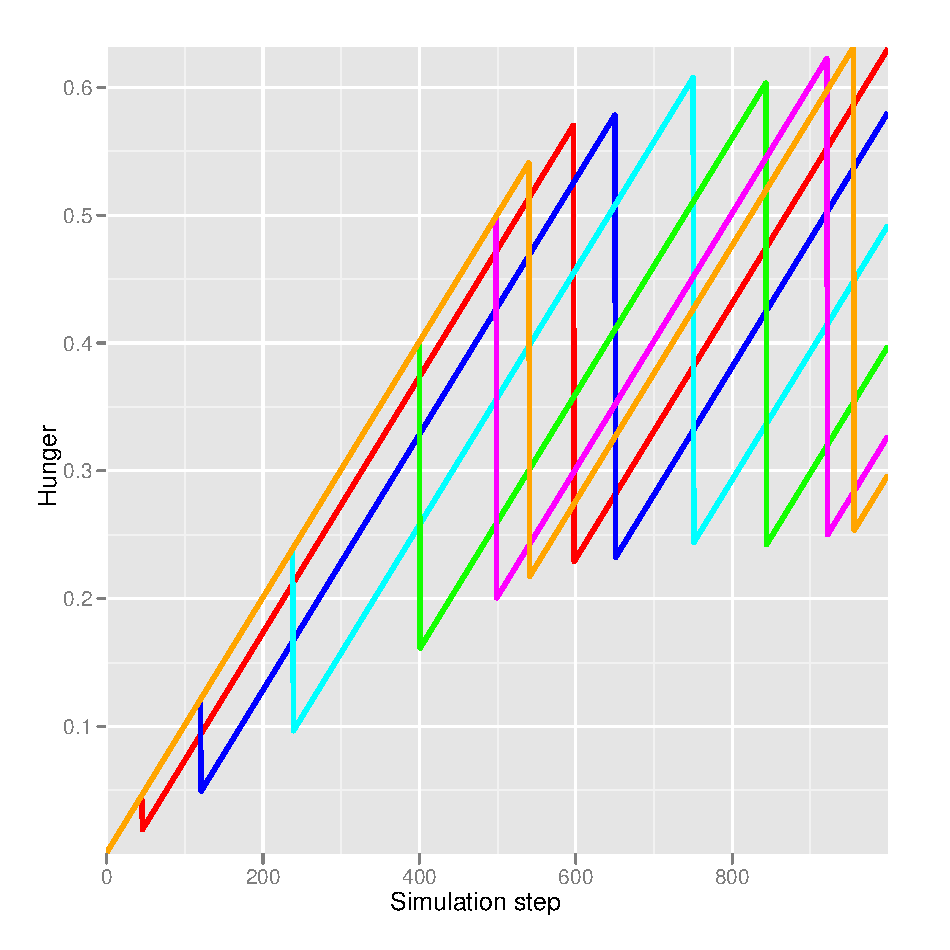
\includegraphics[scale=0.4]{diagrams/experiments/single_agent.eps}    
  \caption{An example of agent's first 1000 steps showing the needs for each kind of food.}
  \label{experiments:singleagent}
\end{figure}

\section{Homogeneus agent set comparision with communication}

In this experiment I will compare avarage life span and efficiency of groups which contains of agents with only single type of memory. Thereby you can see which of the used memory implementation works better in memory homogeneus environment.

What I assume is the \emph{random agents} are about to expire almost immediately as they had no chance to find all the food. While the \emph{PR agents} should approach their goals easily, thereby they will stay alive. Both results of \emph{GNG agent} and \emph{grid agent} are matters of the experiment and I can only expect them not to be worse than \emph{random agent} and not to be better than \emph{PR agent}.     

\subsection{Random agent}   

As for the random agents I assumed that they will immediately pass away without communication. And as you can see in \ref{experiments:random-silent} it happened to be true. 

\begin{figure}
  \centering                                
  \includegraphics[scale=0.4]{diagrams/experiments/random_silent.eps}    
  \caption{Random agent \emph{without communication} fades out quickly.}
  \label{experiments:random-silent}
\end{figure}    

On the other hand, if I allow them to communicate with each other it might happen they improve their chances. Although they will not last through the entire simulation (see \ref{experiments:gng-grid-pr-random}), the result is that they have managed to slow down [it] (see \ref{experiments:random-start}).

\begin{figure}
  \centering                                
  \includegraphics[scale=0.4]{diagrams/experiments/random.eps}    
  \caption{Random agent with communication manages to survive several thousand steps (see \ref{experiments:random-start}).}
  \label{experiments:gng-grid-pr-random}
\end{figure}             

\begin{figure}
  \centering                                
  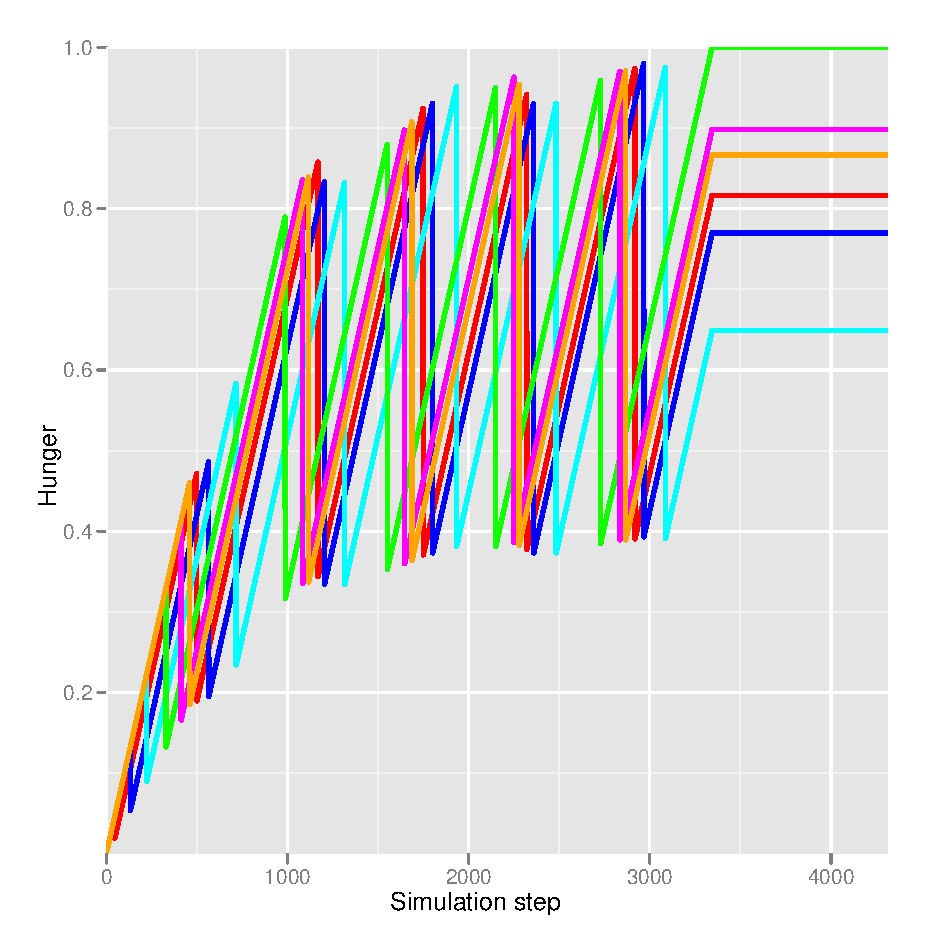
\includegraphics[scale=0.4]{diagrams/experiments/random_start.eps}    
  \caption{A beginning of life of a random agent with communication.}
  \label{experiments:random-start}
\end{figure}        

\subsection{PR agent}

In case of the \emph{pure reactive agents} there is not much to compare between simulation with and without the communication, because the communication is not used since the PR agents see all the environment. So both graphs \ref{experiments:pr} and \ref{experiments:pr-silent} are the same.

\begin{figure}
  \centering                                
  \includegraphics[scale=0.4]{diagrams/experiments/pr.eps}    
  \caption{PR agent with communication.}
  \label{experiments:pr}
\end{figure} 

\begin{figure}
  \centering                                
  \includegraphics[scale=0.4]{diagrams/experiments/pr_silent.eps}    
  \caption{PR agent without communication.}
  \label{experiments:pr-silent}
\end{figure} 

\subsection{GNG agent}

GNG agents need more information to be able to learn and to survive that is why I do not expect them to deal with it well. In case of a simulation without communication they might end up similarly to random agents, they should do better if they communicate.

\begin{figure}
  \centering                                
  \includegraphics[scale=0.4]{diagrams/experiments/gng.eps}    
  \caption{GNG agent with communication.}
  \label{experiments:gng}
\end{figure} 

\begin{figure}
  \centering                                
  \includegraphics[scale=0.4]{diagrams/experiments/gng_silent.eps}    
  \caption{GNG agent without communication.}
  \label{experiments:gng-silent}
\end{figure} 

\subsection{Grid agent}            

I assumed they will do simirarly to GNG agent, i.e. they fail to survive without communication, which assumption ended up to be wrong. 

I have run 20 simulations with grid agents to verify the probability of learning the environment.

%8,8,1,9,7,6,8,1,12,3,5,3,4,2,2,4,7,5,6,12

\begin{center}   
  \emph{mean}=5.56, \emph{median}=5.5, \emph{min}=1, \emph{max}=12                 
\end{center}

\begin{figure}
  \centering                                
  \includegraphics[scale=0.4]{diagrams/experiments/grid.eps}    
  \caption{Grid agent with communication.}
  \label{experiments:gng}
\end{figure} 

\begin{figure}
  \centering                                
  \includegraphics[scale=0.4]{diagrams/experiments/grid_silent.eps}    
  \caption{Grid agent without communication.}
  \label{experiments:gng-silent}
\end{figure} 

\section{Mixed environment}
                                                                                
\subsection{GNG+Grid+PR+Random agents}

Having all agent kinds together in the environment leads to a stable simulation.
            
\begin{center}   
  \begin{tabular}{l*{6}{c}r}
  Agent kind        & median & mean & min & max \\
  \hline
  GNG agents        & 0.7 & 0.699 & 0.57 & 0.86  \\
  Grid agents       & 0.7 & 0.697 & 0.54 & 0.83  \\   
  PR agents         & 0.69 & 0.689 & 0.55 & 0.81 \\  
  Random agents     & 0.7 & 0.704 & 0.57 & 0.87  \\
  All agents        & 0.7 & 0.698 & 0.54 & 0.87  \\ 
  \end{tabular}                  
\end{center}
 
\begin{center}
  \begin{tabular}{l*{6}{c}r}
  Agent kind        & median & mean & min & max \\
  \hline
  GNG agents        & 1 & 1 & 1 & 1  \\
  Grid agents       & 0.61 & 0.721 & 0.47 & 1  \\   
  PR agents         & 0.58 & 0.576 & 0.44 & 0.68 \\  
  Random agents     & 1 & 1 & 1 & 1  \\
  All agents        & 1 & 0.824 & 0.44 & 1  \\ 
  \end{tabular}                    
\end{center}

%[1] "gng-grid-pr-random gng median 0.7 mean 0.698904096385542 min 0.57 max 0.86"
%[1] "gng-grid-pr-random grid median 0.7 mean 0.697301204819277 min 0.54 max 0.83"
%[1] "gng-grid-pr-random pr median 0.69 mean 0.68933734939759 min 0.55 max 0.81"
%[1] "gng-grid-pr-random random median 0.7 mean 0.704657124957833 min 0.57 max 0.87" 
%[1] "gng-grid-pr-random all median 0.7 mean 0.697550029517717 min 0.54 max 0.87"

%[1] "gng-grid-pr-random_silent gng median 1 mean 1 min 1 max 1"
%[1] "gng-grid-pr-random_silent grid median 0.61 mean 0.721167710843373 min 0.47 max 1"
%[1] "gng-grid-pr-random_silent pr median 0.58 mean 0.575706712929497 min 0.44 max 0.68"
%[1] "gng-grid-pr-random_silent random median 1 mean 1 min 1 max 1"  
%[1] "gng-grid-pr-random_silent all median 1 mean 0.824215611860098 min 0.44 max 1"

\begin{figure}
  \centering                                
  \includegraphics[scale=0.4]{diagrams/experiments/gng-grid-pr-random.eps}    
  \caption{GNG, grid, PR and random agents together. Owing to PR agents and the communication they all do well.}
  \label{experiments:gng-grid-pr-random}
\end{figure}

%\begin{figure}
%  \centering                                
%  \includegraphics[scale=0.5]{diagrams/experiments/gng-grid-pr-random_silent.eps}    
%  \caption{GNG, grid, PR and random agents together.}
%  \label{experiments:gng-grid-pr-random-silent}
%\end{figure}
                                       
\subsection{GNG+Grid+Random agents}
             
\begin{center}
  \begin{tabular}{l*{6}{c}r}
  Agent kind        & median & mean & min & max \\
  \hline
  GNG agents        & 0.69 & 0.691 & 0.52 & 0.86  \\
  Grid agents       & 0.7 & 0.700 & 0.55 & 0.87  \\   
  Random agents     & 0.7 & 0.702 & 0.55 & 0.85  \\
  All agents        & 0.7 & 0.698 & 0.52 & 0.87  \\ 
  \end{tabular}                                
\end{center}

\begin{center} 
  \begin{tabular}{l*{6}{c}r}
  Agent kind        & median & mean & min & max \\
  \hline
  GNG agents        & 1 & 1 & 1 & 1  \\
  Grid agents       & 1 & 0.747 & 0.39 & 1  \\   
  Random agents     & 1 & 1 & 1 & 1  \\
  All agents        & 1 & 0.916 & 0.39 & 1  \\ 
  \end{tabular}                                        
\end{center}

%[1] "gng-grid-random gng median 0.69 mean 0.69148588571222 min 0.52 max 0.86"
%[1] "gng-grid-random grid median 0.7 mean 0.699864820905772 min 0.55 max 0.87"
%[1] "gng-grid-random random median 0.7 mean 0.702296598836159 min 0.55 max 0.85"  
%[1] "gng-grid-random all median 0.7 mean 0.697882435151384 min 0.52 max 0.87"

%[1] "gng-grid-random_silent gng median 1 mean 1 min 1 max 1"
%[1] "gng-grid-random_silent grid median 1 mean 0.747429428561102 min 0.39 max 1"
%[1] "gng-grid-random_silent random median 1 mean 1 min 1 max 1"           
%[1] "gng-grid-random_silent all median 1 mean 0.915809809520367 min 0.39 max 1"

\begin{figure}
  \centering                                
  \includegraphics[scale=0.4]{diagrams/experiments/gng-grid-random.eps}    
  \caption{GNG, grid, PR agents together.}
  \label{experiments:gng-grid-pr-random}
\end{figure} 
                                       
\subsection{GNG+Grid agents}

\begin{center} 
  \begin{tabular}{l*{6}{c}r}
  Agent kind        & median & mean & min & max \\
  \hline
  GNG agents        & 0.72 & 0.715 & 0.5 & 0.89  \\   
  Grid agents       & 0.72 & 0.721 & 0.57 & 0.89  \\  
  All agents        & 0.72 & 0.718 & 0.5 & 0.89  \\
  \end{tabular}                       
\end{center}

\begin{center}
  \begin{tabular}{l*{6}{c}r}
  Agent kind        & median & mean & min & max \\
  \hline
  GNG agents        & 1 & 1 & 1 & 1  \\   
  Grid agents       & 1 & 0.755 & 0.4 & 1  \\  
  All agents        & 1 & 0.877 & 0.4 & 1  \\
  \end{tabular}                                 
\end{center}

%[1] "gng-grid gng median 0.72 mean 0.714870602409639 min 0.5 max 0.89"
%[1] "gng-grid grid median 0.72 mean 0.721010337100311 min 0.57 max 0.89" 
%[1] "gng-grid all median 0.72 mean 0.717940506740883 min 0.5 max 0.89"

%[1] "gng-grid_silent gng median 1 mean 1 min 1 max 1"
%[1] "gng-grid_silent grid median 1 mean 0.755093371244066 min 0.4 max 1" 
%[1] "gng-grid_silent all median 1 mean 0.877545210298671 min 0.4 max 1"

\begin{figure}
  \centering                                
  \includegraphics[scale=0.4]{diagrams/experiments/gng-grid.eps}    
  \caption{GNG and grid agents together.}
  \label{experiments:gng-grid-pr-random}
\end{figure}

